\chapter{Shrinkage Methods} \label{ch:shrinkageMethods}
Before we talked about methods that can be used to select the best subset of predictors. Shrinkage Methods regularizes or penalties the coefficient by shrinking the coefficients towards zero. Using this techniques that can reduce the variance. 

\section{Theory}
\subsection{Vector norm}
A norm is a function that gives a positive length to each vector in a vector space.

\noindent Using the P-norm$ \lVert X \rVert_p = ( \sum_{i=1}^{n}|x_i|^p  )^1/p $ \textbf{ref til wiki Norm(mathematics)}. If we set $ p = 1 $ we get the first norm also called the Manhattan norm. It got it's name because it works in a similar to how a taxi would drive in New York City always in a grid-like route 1 block the east then 2 block to the north. The second norm is called Euclidean distance and that is the distance in a straight line just as a bird would fly. Both norms can be seen visually on Figure \ref{fig:normfirstsecond}.

\begin{figure}[H]
	\centering
	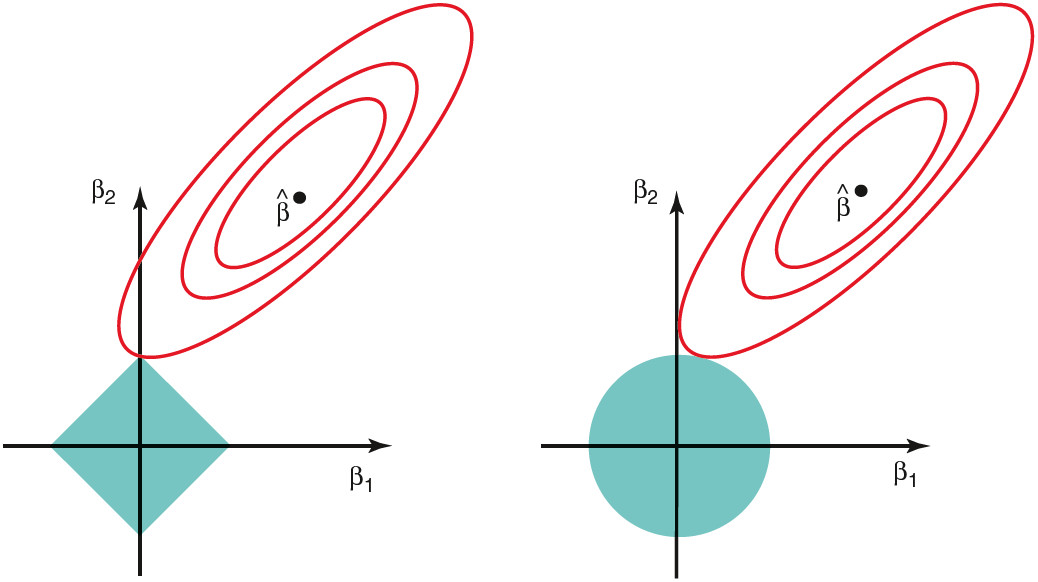
\includegraphics[width=0.6\textwidth]{shrinkageMethods/fig/normsL1_L2.jpg}
	\caption{The red eclipse shows the concurs of ridge (left) and lasso (right) regression. The blue areas are constraint regions for the first and second norm. Notice that lasso intersects the constraint region at an axis, whereas ridge does not.}
	\label{fig:normfirstsecond}
\end{figure}

\subsection{Ridge regression}
The formula for Ridge regression can be seen in \ref{fo:RidgeRegression}. In blue we have the residual sum of square (RSS) term and in red we have the regularize or penalty term. The penalty term is small when $\beta_1, . ,\beta_p$ are close to zero and it has the effect of shrinking or penalizing the estimates of the coefficients $\beta_j$ towards zero. $\lambda$ also called a tuning parameter decides how much impact the two terms get. If $\lambda = 0$ then we will only get least squares estimates, but as $ \lambda \to \infty$ the penalty terms influence will increase and therefore the coefficients will approach zero. This means that the results will be different depending on the chosen $\lambda$ so for getting a good result picking the right $\lambda$ is important.

\noindent The penalty term only apply to the slope, not the intercept. $\lambda$ in in \ref{fo:RidgeRegression} control the degree of penalty.
\begin{align}\label{fo:RidgeRegression}
\color{blue} \sum_{i=1}^{n} ( y_i - \beta_0 - \sum_{j=1}^{p} \beta_j x_i,j )^2 \color{black} + \color{red} \lambda \sum_{j=1}^{p} \beta^2_j 
\end{align}
The reason to Ridge regression over least squares is found in the bias-variance
trade-off. This is because as our $\lambda$ gets bigger the complexity of the ridge regression fit decreases leading to less variance but more bias.

\subsection{The lasso regression}
The formula for least absolute shrinkage and selection operator, also called Lasso, can be seen in figure \ref{foTheLasso}. The blue part of the equation is the RSS (the ) and the red part is the penalty. The lasso regression has a advantage over Ridge regression because of the way the penalty term works. In Ridge it will include all $p_i$ predictors because the $\lambda \sum_{j=1}^{p} \beta^2_j$ only shrink all of the coefficients towards zero but not setting any of them to zero. In lasso we use as E \_ 1 norm of a coefficient vector $\beta$ is given by $ \lVert \beta_1 \rVert = \sum | \beta_j |$ which makes some of the coefficient estimates to be exactly zero when the tuning parameter $\lambda$ is large enough.
\begin{align}\label{fo:TheLasso}
\color{blue} \sum_{i=1}^{n} ( y_i - \beta_0 - \sum_{j=1}^{p} \beta_j x_i,j )^2 \color{black} +  \color{red} \lambda \sum_{j=1}^{p} |\beta_j|
\end{align}
Because the lasso regression removes some of the coefficients, lasso models are generally easier to understand than Ridge regression ones because they are  more sparse with a reduced complexity. Lasso models involve only a subset of the variables. As before selecting a good $\lambda$ is again important here.

\subsection{Comparing ridge and lasso regression}

From equations \ref{fo:RidgeRegression} and \ref{fo:TheLasso} we see that a Lasso regression model could potentially end up with less variables than Ridge regression, since the coefficients can be forced to equal zero, because of the $\ell_1$ penalty. This is called sparsity. You would typically use Ridge regression to prevent over-fitting, since it keeps all features, but can prove less useful with a large number of features (\textit{p} > \textit{n}) On the other hand, Lasso is useful when you have many features and provides you with a more sparse model that could prove a computational advantage. In terms of prediction error, Ridge regression generally performs better in terms of bias, variance and MSE when the predictors are related to the response, that is none of the true coefficients are zero. However if the response is just a subset of the original predictors, we tend to get better results with Lasso regression.

\section{Results}
In lab 6.6.1 we use Ridge Regression on the hitters dataset. We use scikit-lean and their implmeation. After loading the data we found that some players had missing salary, therefor these were dropped. The data also contained some string values and usingf'' pandas we have converted them into dummy variables.  
\begin{figure}[H]
	\centering
	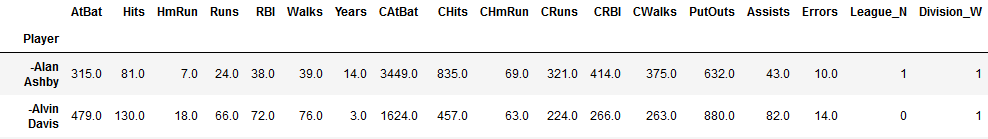
\includegraphics[width=0.8\textwidth]{shrinkageMethods/fig/data.png}
	\caption{The data after removing missing values and making strings into dummy variables }
	\label{fig:normfirstsecond}
\end{figure}
Then we split our data into a training and test set and we try to run Ridge Regression with a alpha of 4 and display our mean squared error.
\begin{lstlisting}[language=Python]
ridge = Ridge(alpha=4)
ridge.fit(X_train, y_train)
result = ridge.predict(X_test)
metrics.mean_squared_error(y_test, result)
134512.83820473132
\end{lstlisting}
After that we display some of the coefficients.
\begin{lstlisting}[language=Python]
pd.Series(ridge.coef_.flatten(), index=X.columns)
AtBat          -2.185390
Hits            7.392346
HmRun          -2.666724
\end{lstlisting}
If we run the same code again but with a alpha that is very large $10^10$ then are coefficients get even smaller.
\begin{lstlisting}[language=Python]
AtBat          5.135079e-04
Hits           1.771301e-04
HmRun          2.568334e-05
-- omitted --
\end{lstlisting}
And our MSE also gets even higher.
\begin{lstlisting}[language=Python]
211698.60251243794
\end{lstlisting}
As discussed in the theory and see just before picking the right alpha part of this is important. We will now use cross validation to pick the best alpha using scikit learn's RidgeCV. That is Ridge regression with built-in cross-validation.
\begin{lstlisting}[language=Python]
alphas = 10**np.linspace(100,-4,1000)
ridgecv = RidgeCV(alphas=alphas, scoring='neg_mean_squared_error')
ridgecv.fit(scale(X_train), y_train)
ridgecv.alpha_
2.3570694139967037
\end{lstlisting}
Now we will use the alpha we found using  cross validation and check our result.
\begin{lstlisting}[language=Python]
ridge = Ridge(2.3570694139967037)
ridge.fit(X_train, y_train)
result = ridge.predict(X_test)
metrics.mean_squared_error(y_test, result)
134355.75204499933
\end{lstlisting}
Using a plot we can also see the trend here that the coefficients move toward zero.
\begin{figure}[H]
	\centering
	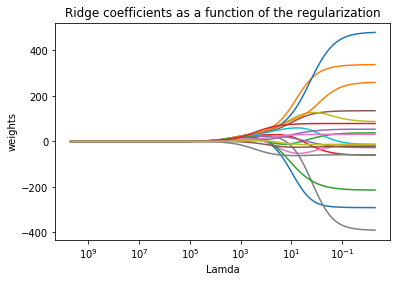
\includegraphics[width=0.5\linewidth]{shrinkageMethods/fig/plot}
	\caption{Ridge regression on the hitters dataset}
	\label{fig:plot}
\end{figure}
In lab 6.6.2 we use The Lasso and the same steps to prepere the dataset as before. We need to select the best alpha and to do this we use LassoCV that has cross validation built ind.
\begin{lstlisting}[language=Python]
alphas = 10**np.linspace(100,-20,100)
lassoCV = LassoCV(alphas=alphas)
lassoCV.fit(X_train, y_train)
lassoCV.alpha_
1072.2672220103254
\end{lstlisting}
As we can see some of the coefficients here are zero just as we described in the theory section.
\begin{lstlisting}[language=Python]
pd.Series(lassoCV.coef_.flatten(), index=X.columns)
AtBat          0.729684
Hits           0.000000
HmRun         -0.000000
Runs           0.000000
-- omitted --
\end{lstlisting}